\documentclass[11p]{article}
\usepackage[a4paper,bindingoffset=0.2in,%
left=1in,right=1in,top=1in,bottom=1in,%
footskip=.25in]{geometry}
\usepackage{amsmath}
\usepackage{mathtools}
\usepackage{amssymb}
\usepackage{graphicx}
\usepackage{float}
\usepackage{subcaption}

\newcommand{\CR}{\textup{CR}}
\newcommand{\NC}{\textup{NC}}
\renewcommand{\d}[1]{\ensuremath{\,\textup{d} #1}}

\DeclareMathOperator{\LS}{\operatorname{LS}}

\begin{document}
	\noindent The nonconforming problem minimizes the discrete energy $E_\NC$ in $\CR_0^1(\mathcal{T})$ with
	\begin{align*}
		E_\NC(v_\CR) \coloneqq \frac{\alpha}{2}\|v_\CR\|^2_{L^2(\Omega)} + |v_\CR|_{1,1,\NC} - \int_{\Omega} f v \d{x}.
	\end{align*}
	The adaptive algorithm employs the following error estimator
	\begin{align*}
		\eta^2(T) \coloneqq \underbrace{|T|^{1/2}\|f - \alpha u_\CR\|^2_{L^2(\Omega)}}_{\mu(T)} + \underbrace{|T|^{\beta/2}\sum_{F \in \mathcal{F}(T)} \|[u_\CR]_F\|_{L^1(F)}}_{\xi(T)}
	\end{align*}
	for any $T \in \mathcal{T}$. The stopping criteria is set to $\epsilon = 10^{-5}$ in the following examples.
	
	\section{Example with exact solution}
	\section{Example with discontinuity set}
	Let $\Omega = (-1,1)^2$, $\alpha = 100$ and $f \in L^2(\Omega)$ with
	\begin{align*}
		f(x) = \begin{cases}
			100 &\mbox{if } |x|_\infty < 1/2,\\
			0 &\mbox{otherwise}.
		\end{cases}
	\end{align*}
	\begin{figure}[H]
		\centering
		\begin{subfigure}{0.5\linewidth}
			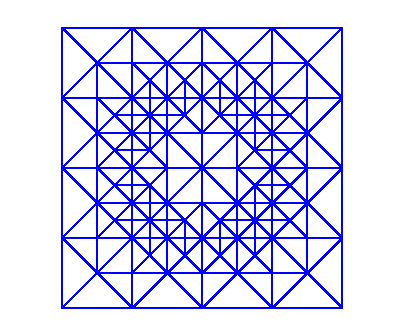
\includegraphics[width=\linewidth]{figures/discSet/adaptTriangulation/adaptTriangulationLevel4} 
			\caption{117 nodes}
		\end{subfigure}\hfill
		\begin{subfigure}{0.5\linewidth}
			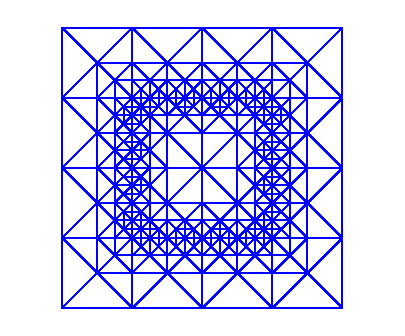
\includegraphics[width=\linewidth]{figures/discSet/adaptTriangulation/adaptTriangulationLevel5}
			\caption{256 nodes}
		\end{subfigure}
		
		\begin{subfigure}{0.5\linewidth}
			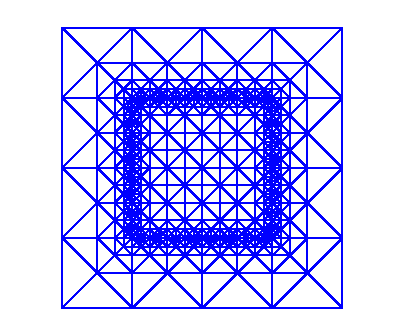
\includegraphics[width=\linewidth]{figures/discSet/adaptTriangulation/adaptTriangulationLevel6}
			\caption{550 nodes}
		\end{subfigure}\hfill
		\begin{subfigure}{0.5\linewidth}
			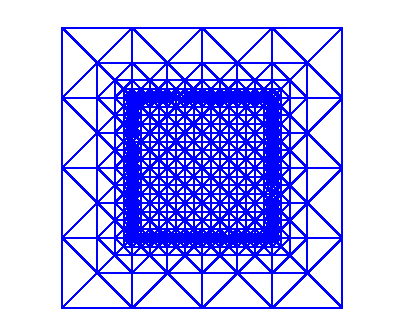
\includegraphics[width=\linewidth]{figures/discSet/adaptTriangulation/adaptTriangulationLevel7}
			\caption{1138 nodes}
		\end{subfigure}
		\caption{successive adaptively generated meshes with $\beta = 1$}
	\end{figure}

	\begin{figure}[H]
		\centering
		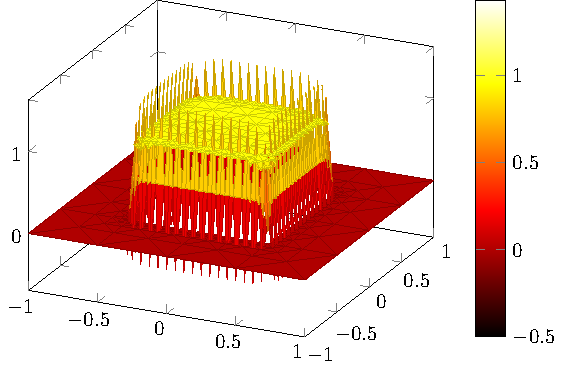
\includegraphics[width=12cm]{figures/discSet/discSolution/discSolution.pdf}
		\caption{discrete solution on an adaptively refined mesh ($\beta = 1$) with 550 nodes}
	\end{figure}

	\begin{figure}[H]
		\centering
		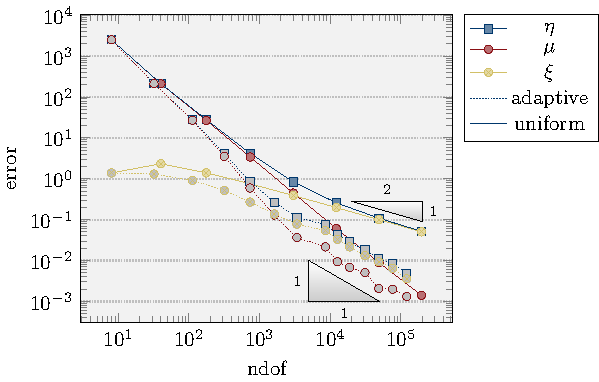
\includegraphics[width=14cm]{figures/discSet/convHistoryPlot/convergence.pdf}
		\caption{convergence history plot for $\eta$, $\mu$ and $\xi$ with $\beta = 1$}
	\end{figure}

	\begin{figure}[H]
		\centering
		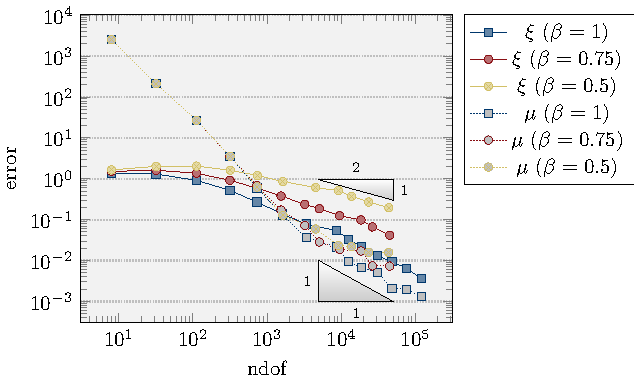
\includegraphics[width=14cm]{figures/discSet/compBeta/compBeta.pdf}
		\caption{convergence history plot for $\mu$ and $\xi$ with different $\beta$}
	\end{figure}
	
	\section{Application to image processing}
	The right hand side $f$ represents the greyscale of the image in the left plot of times the factor $\alpha = 10000$ where the greyscale is some real number in $[0,1]$. The original image has a size of 256x256 pixels and is displayed  in . The image is scaled to the domain $\Omega = (0,1)^2$.
	
	\begin{figure}[H]
		\centering
		\begin{subfigure}{0.45\linewidth}
			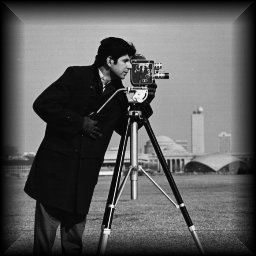
\includegraphics[width=\linewidth]{figures/imgProcessing/example.png}
		\end{subfigure}\quad
		\begin{subfigure}{0.45\linewidth}
			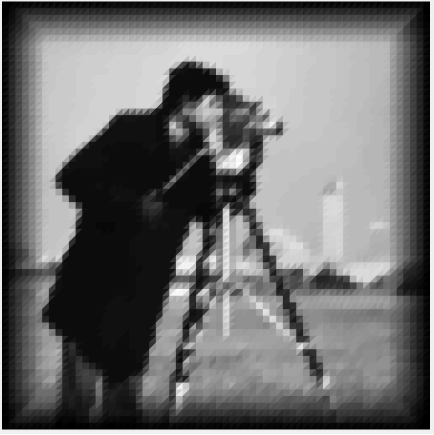
\includegraphics[width=\linewidth]{figures/imgProcessing/imgUniformLevel7}
		\end{subfigure}
		\caption{original image (left) on a uniform mesh with 66049 nodes and generated image (right) on a uniform mesh with 16641 nodes}
	\end{figure}

	\begin{figure}[H]
		\centering
		\begin{subfigure}{0.45\linewidth}
			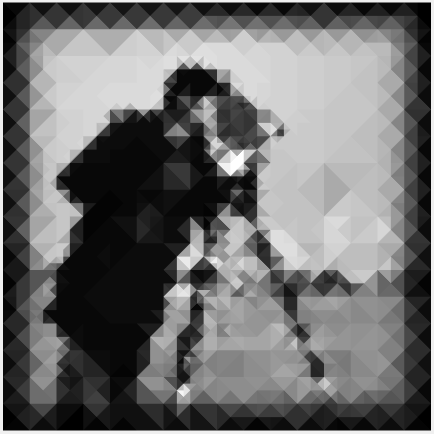
\includegraphics[width=\linewidth]{figures/imgProcessing/imgAdaptiveLevel12.png}
			\caption{850 nodes}
		\end{subfigure}\quad
		\begin{subfigure}{0.45\linewidth}
			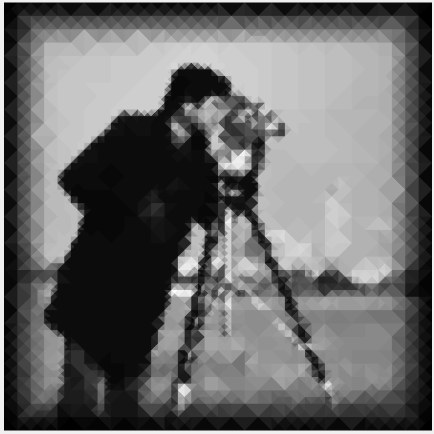
\includegraphics[width=\linewidth]{figures/imgProcessing/imgAdaptiveLevel14}
			\caption{2091 nodes}
		\end{subfigure}\vspace{1em}
		
		\begin{subfigure}{0.45\linewidth}
			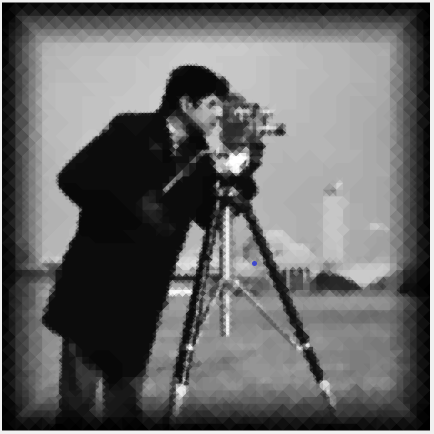
\includegraphics[width=\linewidth]{figures/imgProcessing/imgAdaptiveLevel16.png}
			\caption{5527 nodes}
		\end{subfigure}\quad
		\begin{subfigure}{0.45\linewidth}
			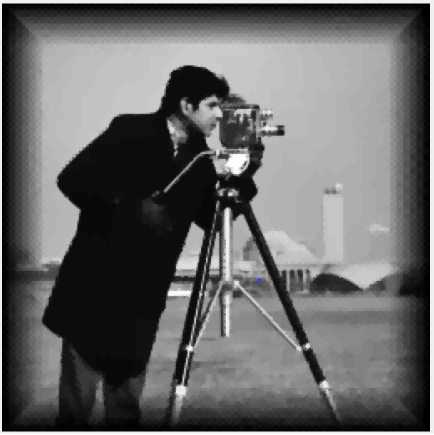
\includegraphics[width=\linewidth]{figures/imgProcessing/imgAdaptiveLevel18}
			\caption{13955 nodes}
		\end{subfigure}
		\caption{generated images on adaptive meshes after 12 (upper left), 14 (upper right), 16 (bottom left) and 18 (bottom right) iterations of the adaptive algorithm}
	\end{figure}

	\begin{figure}[H]
		\centering
		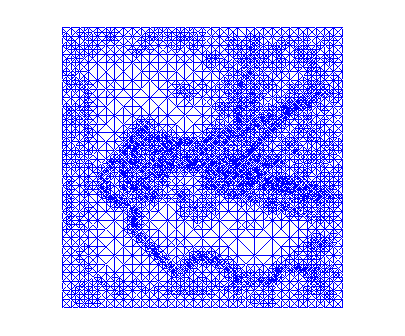
\includegraphics[trim = 0.9cm 0.35cm 0.9cm 0.2cm, width=\linewidth, angle=-90]{figures/imgProcessing/adaptTriangulation/adaptTriangulationLevel16}
		\caption{adaptive mesh with 5527 nodes}
	\end{figure}
	
	\begin{figure}[H]
		\centering
		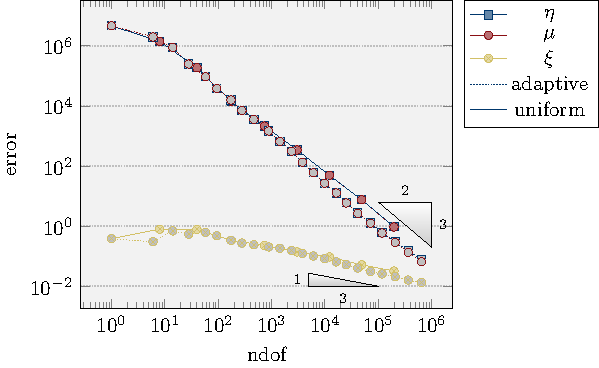
\includegraphics[width=14cm]{figures/imgProcessing/convHistoryPlot/convergence.pdf}
		\caption{convergence history plot for $\eta$, $\mu$ and $\xi$}
	\end{figure}

	\section{Example with a noisy image}
	
\end{document}